\documentclass[11pt, dvipsnames, handout]{beamer}
\newtoggle{full}
\settoggle{full}{true}

\newtoggle{covered}
\settoggle{covered}{false}

\newtoggle{presentable}
\settoggle{presentable}{false}

\newtoggle{dualscreen}
\settoggle{dualscreen}{false}

\usepackage{pgfplots}
%\pgfplotsset{compat = newest}

\usepackage{pgfpages}

\setbeamertemplate{note page}{\pagecolor{yellow!5}\vfill \insertnote \vfill}
\usepackage{collect}
\definecollection{notes}
\newcounter{notestaken}

\usepackage{xpatch}

\usepackage{ulem}

\usepackage[framemethod=tikz]{mdframed}

\usepackage{scalerel}
\usepackage{calc}

%\usepackage{enumitem}
\setlength\fboxsep{.2em}

\usepackage{graphicx} % Allows including images
\usepackage{booktabs} % Allows the use of \toprule, \midrule and \bottomrule in tables

\xpatchcmd{\itemize}
  {\def\makelabel}
  {\setlength{\itemsep}{0.65 em}\def\makelabel}
  {}
  {}


\xpatchcmd{\beamer@enum@}
  {\def\makelabel}
  {\setlength{\itemsep}{0.65 em}\def\makelabel}
  {}
  {}


%\makeatletter
%\renewcommand{\itemize}[1][]{%
%  \beamer@ifempty{#1}{}{\def\beamer@defaultospec{#1}}%
%  \ifnum \@itemdepth >2\relax\@toodeep\else
%    \advance\@itemdepth\@ne
%    \beamer@computepref\@itemdepth% sets \beameritemnestingprefix
%    \usebeamerfont{itemize/enumerate \beameritemnestingprefix body}%
%    \usebeamercolor[fg]{itemize/enumerate \beameritemnestingprefix body}%
%    \usebeamertemplate{itemize/enumerate \beameritemnestingprefix body begin}%
%    \list
%      {\usebeamertemplate{itemize \beameritemnestingprefix item}}
%      {%
%        \setlength\topsep{1em}%NEW
%        \setlength\partopsep{1em}%NEW
%        \setlength\itemsep{1em}%NEW
%        \def\makelabel##1{%
%          {%
%            \hss\llap{{%
%                \usebeamerfont*{itemize \beameritemnestingprefix item}%
%                \usebeamercolor[fg]{itemize \beameritemnestingprefix item}##1}}%
%          }%
%        }%
%      }
%  \fi%
%  \beamer@cramped%
%  \raggedright%
%  \beamer@firstlineitemizeunskip%
%}
%
%
%
%
%
%\makeatother

%\setlist[beamer@enum@]{topsep=1 em}
%\let\origcheckmark\checkmark %screw you dingbat
%\let\checkmark\undefined %screw you dingbat
%\usepackage{dingbat} 
%\let\checkmark\origcheckmark %screw you dingbat






%\usepackage{fontawesome}

\usepackage{mathtools}
\usepackage{etoolbox, calculator}

\usepackage{xcolor}
\usepackage{tikz}
\usetikzlibrary{arrows.meta}
\usetikzlibrary{calc}
\usepackage[nomessages]{fp}
\usepackage{transparent}
\usepackage{accsupp}
%\usepackage{color, xcolor}

%colorblind-friendly palette
%\definecolor{dblue}{RGB}{51,34,136}
\definecolor{lblue}{RGB}{136,204,238}
%\definecolor{green}{RGB}{17,119,51}
\definecolor{tan}{RGB}{221,204,119}
%\definecolor{mauve}{RGB}{204,102,119}

\usepackage{tcolorbox}



\usepackage{xifthen}
\usepackage{nicefrac}
\usepackage{amsmath}
\usepackage{amsthm}
\usepackage{amssymb}
\theoremstyle{definition}
\newtheorem*{define}{Definition}
\newtheorem*{recall}{Recall}


\DeclareMathOperator{\tr}{tr}

\usepackage{multicol}
%\setlength{\columnsep}{1cm}

\usepackage{tablists, amsmath,vwcol, cancel, polynom}
\usetikzlibrary{shapes, patterns, decorations.shapes}
%\usepackage{tikzpeople}
\tikzstyle{vertex}=[shape=circle, minimum size=2mm, inner sep=0, fill]
\tikzstyle{opendot}=[shape=circle, minimum size=2mm, inner sep=0, fill=white, draw]

% common math quick commands
\newcommand{\nicedd}[2]{\nicefrac{\text{d}#1}{\text{d}#2}}
\newcommand{\dd}[2]{\dfrac{\text{d}#1}{\text{d}#2}}
\newcommand{\pd}[2]{\dfrac{\partial #1}{\partial#2}}
\renewcommand{\d}[1]{\text{d}#1}
\newcommand{\ddn}[3]{\dfrac{\text{d}^{#3}#1}{\text{d}#2^{#3}}}
\newcommand{\pdn}[3]{\dfrac{\partial^{#3}#1}{\partial#2^{#3}}}
\newcommand{\p}[0]{^{\prime}}
\newcommand{\pp}[0]{^{\prime\prime}}
\newcommand{\op}[2][\text{L}]{#1 \left[ #2 \right]}

\newcommand{\lap}[1]{\mathcal{L}\left\{#1\right\}}
\newcommand{\lapinv}[1]{\mathcal{L}^{-1}\left\{#1\right\}}
\newcommand{\lapint}[1]{\int_0^\infty e^{-st}#1dt}
\newcommand{\evalat}[2]{\Big|_{#1}^{#2}}

\newcommand{\paren}[1]{ \left( #1 \right)}

\newcommand{\haxis}[4][\normcolor]{\draw[#1, <->] (-#2,0)--(#3,0) node[right]{$#4$}; }


\newcommand{\axis}[4]{\draw[\normcolor, <->] (-#1,0)--(#2,0) 
node[right]{$x$};
\draw[help lines, <->] (0,-#3)--(0,#4) node[above]{$y$};}

\newcommand{\laxis}[6]{\draw[<->] (-#1,0)--(#2,0) 
node[right]{$#5$};
\draw[ <->] (0,-#3)--(0,#4) node[above]{$#6$};}
\newcommand{\xcoord}[2]{
	\draw (#1,.2)--(#1,-.2) node[below]{$#2$};}
\newcommand{\textnode}[3]{
	\draw (#1,#2) node[below]{$#3$};}
	
\newcommand{\nxcoord}[2]{
	\draw (#1,-.2)--(#1,.2) node[above]{$#2$};}
\newcommand{\ycoord}[2]{
	\draw (.2,#1)--(-.2,#1) node[left]{$#2$};}
\newcommand{\nycoord}[2]{
	\draw (-.2,#1)--(.2,#1) node[right]{$#2$};}
\newcommand{\dlim}{\displaystyle\lim}
\newcommand{\dlimx}[1]{\displaystyle\lim_{x \rightarrow #1}}
\newcommand{\stickfig}[2]{
	\draw (#1,#2) arc(-90:270:2mm);
	\draw (#1,#2)--(#1,#2-.5) (#1-.25,#2-.75)--(#1,#2-.5)--(#1+.25,#2-.75) (#1-.2,#2-.2)--(#1+.2,#2-.2);}	

%\newcounter{example}
%\setcounter{example}{1}
%\newcounter{preFrameExample}
%\AtBeginEnvironment{frame}{\setcounter{preFrameExample}{\value{example}}}
%\newcommand{\ex}[1]{
%	 \setcounter{example}{\value{preFrameExample}}
%	 \textcolor{green}{\small\fbox{Example \arabic{example}: #1}}\\[8pt]
%	\stepcounter{example}}
%\newcommand{\exans}[1]{
%	\SUBTRACT{\value{preFrameExample}}{1}{\n}
%	 \textcolor{green}{\small\fbox{Solution \n: #1}}\\[8pt]}
\mode<presentation> {

% The Beamer class comes with a number of default slide themes
% which change the colors and layouts of slides. Below this is a list
% of all the themes, uncomment each in turn to see what they look like.


\usetheme{CambridgeUS}
\usecolortheme[named=black]{structure}


\newcommand{\studentcolor}[0]{ForestGreen}
\newcommand{\normcolor}[0]{NavyBlue}
\newcommand{\alertcolor}{Red}

\setbeamercolor{normal text}{fg=\normcolor}
\setbeamercolor{frametitle}{fg=\normcolor}
\setbeamercolor{section in head/foot}{fg=Black, bg=Gray!20}
\setbeamercolor{subsection in head/foot}{fg=Green!70!Black, bg=Gray!10}
\setbeamercolor{alerted text}{fg=\alertcolor}
\setbeamerfont{alerted text}{series=\bf}
\setbeamertemplate{enumerate items}[default]
\setbeamercolor{enumerate item}{fg=\normcolor}

\setbeamertemplate{footline} % To remove the footer line in all slides uncomment this line
%\setbeamertemplate{footline}[page number] % To replace the footer line in all slides with a simple slide count uncomment this line

\setbeamertemplate{navigation symbols}{} % To remove the navigation symbols from the bottom of all slides uncomment this line
}

\newcommand{\alertbox}[1]{\tcbox[on line, colframe=\alertcolor, colback=White, left=2pt,right=2pt,top=2pt,bottom=2pt]{\usebeamercolor*{normal text}#1}}


\newcommand{\startstu}{\setbeamercolor{normal text}{fg=\studentcolor}\usebeamercolor*{normal text}\setbeamercolor{enumerate item}{fg=\studentcolor}\usebeamercolor*{enumerate item}}
\newcommand{\stopstu}{\setbeamercolor{normal text}{fg=\normcolor}\usebeamercolor*{normal text}\setbeamercolor{enumerate item}{fg=\normcolor}\usebeamercolor*{enumerate item}}

\newcommand{\takenote}[1]{ \begin{collect}{notes}{}{}{}{}  #1  \end{collect}  \addtocounter{notestaken}{1}} %\ifthenelse{\value{notestaken}>0}{\hrulefill\\}{}

\makeatletter
\newcommand{\cover}{\alt{\beamer@makecovered}{\beamer@fakeinvisible}}
\newcommand{\ucover}[1]{\iftoggle{full}{}{\beamer@endcovered}\stopstu#1\startstu\iftoggle{full}{}{\beamer@startcovered}}
\makeatother

\newcommand{\skippause}{ \addtocounter{beamerpauses}{-1}}
\newcommand{\blockpres}{ \skippause \pause }

\newcommand{\studentify}[1]{\startstu #1  \stopstu }
\newcommand{\student}[1]{\iftoggle{full}{ \pause  \studentify{#1} }{\iftoggle{covered}{\studentify{#1}}{\cover{  #1 }}}}
\newcommand{\cstudent}[1]{\student{\begin{center} #1 \end{center}}}
\newcommand{\fullonly}[1]{\iftoggle{full}{ #1}{}}
\newcommand{\presentonly}[1]{\iftoggle{presentable}{ #1}{}}

\usepackage{xparse}
\usepackage{xifthen}

% shortcuts for commonly-used presentation elements
%\NewDocumentCommand{\slide}{o m}
% {\IfValueTF{#1}{\begin{frame}[t]{#1}}{\begin{frame}[t]} #2 \end{frame}}

\newtoggle{iscovered}

\newcommand{\slide}[2][]{%
%\setcounter{notestaken}{0}
\takenote{#2} 
%\ifthenelse{\equal{#1}{}}{\begin{frame}[t]}{\begin{frame}[t]{#1}} #2 \ifthenelse{\value{notestaken}>0}{ \note{\includecollection{notes}}}{} \end{frame}%
\ifthenelse{\equal{#1}{}}{\begin{frame}[t]}{\begin{frame}[t]{#1}} #2 \iftoggle{covered}{\settoggle{iscovered}{true}}{\settoggle{iscovered}{false}}  \note{ \iftoggle{iscovered}{}{\settoggle{covered}{true}} #2 \iftoggle{iscovered}{}{\settoggle{covered}{false}} } \end{frame}%
%\setcounter{notestaken}{0}
}
\newcommand{\defn}[2][]{%
 \setcounter{listcounter}{0}%
\ifthenelse{\equal{#1}{}}{\begin{block}{Definition}}{\begin{block}{#1 :}}%
 #2 \vspace{0.25em} \ifthenelse{\value{listcounter}>0}{\skippause}{} \pause \end{block}%
}



\newcommand{\arr}[2]{\begin{array}{#1}#2\end{array}}
\newcommand{\mat}[2]{\left[\arr{#1}{#2}\right]}
\newcommand{\carray}[1]{\arr{c}{#1}}
\newcommand{\larray}[1]{\arr{l}{#1}}
\newcommand{\rarray}[1]{\arr{r}{#1}}
\newcommand{\colvec}[1]{\mat{c}{#1}}

\newcommand{\itmz}[1]{\addtocounter{listcounter}{1} \begin{itemize}#1 \end{itemize} }
\newcommand{\subitem}[1]{\addtocounter{listcounter}{1} \begin{itemize} \item #1 \end{itemize}}
%
\newcommand{\enum}[1]{\addtocounter{listcounter}{1} \begin{enumerate} #1  \end{enumerate}  }


\newcommand{\algnlbl}[1]{\begin{align}#1  \end{align}} 
\newcommand{\algn}[1]{\begin{align*}#1  \end{align*}} 
\newcommand{\lgn}[1]{ \action<+->{#1} }
\newcommand{\slgn}[1]{\iftoggle{full}{\action<+->{ \startstu #1 \stopstu}}{ \cover{ #1 } } \takenote{$#1$}}

\newcommand{\chckmrk}{\alert{\checkmark}}

\usepackage{pifont}
\newcommand{\xmark}{\alert{\text{\large \ding{55}}}}

\newcommand{\return}[0]{\raisebox{.5ex}{\rotatebox[origin=c]{180}{$\Lsh$}}}
\usepackage{pbox}
%\newcommand{\ex}[1]{\rotatebox[origin=c]{10}{\uline{ex}}:$\;$\pbox[t][][b]{0.9\linewidth}{#1}}
\newcommand{\ex}[1]{\uline{ex}:$\;$\pbox[t][][t]{0.9\linewidth}{#1}}
\newcommand{\eg}[1]{e.g.,$\;$\pbox[t][][t]{0.9\linewidth}{#1}}
\newcommand{\tikzplot}[8][]{%
\begin{tikzpicture}

\begin{scope}[]%
\clip(-#2,-#4) rectangle (#3,#5);%
#8%
\end{scope}%
\laxis{#2}{#3}{#4}{#5}{#6}{#7}%
#1
\end{tikzpicture}%
}


\newcommand{\cancelslide}[1]{%
\begingroup%
\setbeamertemplate{background canvas}{%
\begin{tikzpicture}[remember picture,overlay]%
\draw[line width=2pt,red!60!black] %
  (current page.north west) -- (current page.south east);%
\draw[line width=2pt,red!60!black] %
  (current page.south west) -- (current page.north east);%
\end{tikzpicture}}%
#1%
\endgroup%
}
\renewcommand{\CancelColor}{\color{red}}
\newcommand{\twocols}[3][0.5]{\begin{columns}\begin{column}{#1\textwidth}#2\end{column}\hspace{1em}\vrule{}\hspace{1em}\begin{column}{#1\textwidth}#3\end{column}\end{columns}}

\newcommand{\twomini}[5][1]{\calculatespace \begin{minipage}[t]{\columnwidth}\begin{minipage}[][#1\contentheight][t]{#2\columnwidth}#4\end{minipage}\hfill\begin{minipage}[][#1\contentheight][t]{#3\columnwidth}#5\end{minipage}\end{minipage}}

\newcommand{\threemini}[7][1]{\calculatespace \begin{minipage}[t]{\columnwidth}\begin{minipage}[][#1\contentheight][t]{#2\columnwidth}#5\end{minipage}\hfill\begin{minipage}[][#1\contentheight][t]{#4\columnwidth}#6\end{minipage}\hfill\begin{minipage}[][#1\contentheight][t]{#3\columnwidth}#7\end{minipage}\end{minipage}}


\newcounter{listcounter}
\setcounter{listcounter}{0}



\newif\ifsidebartheme
\sidebarthemetrue

\newdimen\contentheight
\newdimen\contentwidth
\newdimen\contentleft
\newdimen\contentbottom
\makeatletter
\newcommand*{\calculatespace}{%
\contentheight=\paperheight%
\ifx\beamer@frametitle\@empty%
    \setbox\@tempboxa=\box\voidb@x%
  \else%
    \setbox\@tempboxa=\vbox{%
      \vbox{}%
      {\parskip0pt\usebeamertemplate***{frametitle}}%
    }%
    \ifsidebartheme%
      \advance\contentheight by-1em%
    \fi%
  \fi%
\advance\contentheight by-\ht\@tempboxa%
\advance\contentheight by-\dp\@tempboxa%
\advance\contentheight by-\beamer@frametopskip%
\ifbeamer@plainframe%
\contentbottom=0pt%
\else%
\advance\contentheight by-\headheight%
\advance\contentheight by\headdp%
\advance\contentheight by-\footheight%
\advance\contentheight by4pt%
\contentbottom=\footheight%
\advance\contentbottom by-4pt%
\fi%
\contentwidth=\paperwidth%
\ifbeamer@plainframe%
\contentleft=0pt%
\else%
\advance\contentwidth by-\beamer@rightsidebar%
\advance\contentwidth by-\beamer@leftsidebar\relax%
\contentleft=\beamer@leftsidebar%
\fi%
}
\makeatother



\iftoggle{dualscreen}{\setbeameroption{show notes on second screen=right}}{}
\usetikzlibrary{arrows}
\usetikzlibrary{decorations.markings}

\tikzset{
    set arrow inside/.code={\pgfqkeys{/tikz/arrow inside}{#1}},
    set arrow inside={end/.initial=stealth, opt/.initial={scale=2}},
    /pgf/decoration/Mark/.style={
        mark/.expanded=at position #1 with
        {
            \noexpand\arrow[\pgfkeysvalueof{/tikz/arrow inside/opt}]{\pgfkeysvalueof{/tikz/arrow inside/end}}
        }
    },
    arrow inside/.style 2 args={
        set arrow inside={#1},
        postaction={
            decorate,decoration={
                markings,Mark/.list={#2}
            }
        }
    },
}
\newcommand{\cellheight}{0.6\textheight}
\newcommand{\cellwidth}{.33\columnwidth}
\newcommand{\picheight}{0.6\textheight}
\pgfplotsset{compat = newest}
\begin{document}
\section{Lecture 22}
\subsection{Preamble}


\slide[Recall: Stability of fixed points]{
Solutions flow towards or away from fixed points. \subitem{Stable fixed points attract nearby solutions. \item Unstable fixed points repel nearby solutions.}

\ex{} \[ \dd{y}{t} = y \left( 5-y\right) \]\vfill
\twomini[.5]{.5}{.45}{
Two Fixed Points:
\algn{   y^*&=0 &\text{(unstable)}\intertext{and}
y^*&=5&\text{(stable)}}
}{\vfill
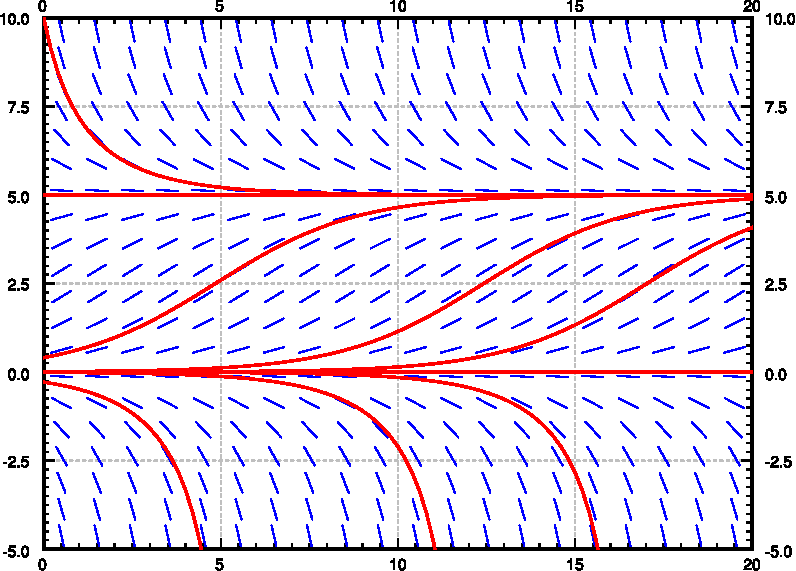
\includegraphics[width=\columnwidth]{images/2-2-logistic-mbx.pdf}
}
}


\subsection{Phase Plane Behaviour}

\slide[Qualitative behaviour of solutions: Stability]{
The origin $\vec{0}$ is always a fixed point for the system  $\dd{}{t}\vec{x} = \mathbf{A}(t) \vec{x}$.
\vfill
Q: Do solutions approach or move away from this fixed point?\\
A: It depends on the eigenvalues, $\lambda$, of $\mathbf{A}$.
\vfill
\student{
\itmz{\item If all $\lambda$'s have ${\rm Re}(\lambda)<0$, solutions approach $\vec{0}$ as $t\to\infty$.\vfill\subitem{\alert{Stable fixed point}}\vfill
\item If any $\lambda$'s have ${\rm Re}(\lambda)>0$, solutions move away from $\vec{0}$  as $t\to\infty$.\vfill\subitem{\alert{Unstable fixed point}}\vfill
\item If a complex conjugate $\lambda$ pairs exists, solutions  exhibit oscillations around $\vec{0}$.\vfill
\subitem{\alert{Spiral fixed point}}} \vfill
}


}
\slide[Classifying Fixed Points]{
The origin $\vec{0}$ is always a fixed point for the system  $\dd{}{t}\vec{x} = \mathbf{A}(t) \vec{x}$.
\vfill

\student{
 If all eigevalues are real and ...\vfill
\itmz{\item they have the same sign, the fixed point is called a \alert{node}\vfill \subitem{All $\lambda\text{'s}<0 \quad \Rightarrow$ \alert{stable node} (sink) \vfill \item All $\lambda\text{'s}>0 \quad \Rightarrow$ \alert{unstable node} (source)}\vfill
\item some $\lambda$'s have opposite signs, the fixed point is called a \alert{saddle}
}
}
}



\slide[Classifying Fixed Points]{
The origin $\vec{0}$ is always a fixed point for the system  $\dd{}{t}\vec{x} = \mathbf{A}(t) \vec{x}$.\vfill
\student{
 If a pair of eigenvalues are complex conjugates, $\lambda_{1,2}=r \pm i \omega$, then  the fixed point is called a \alert{spiral} (or focus).\vfill
\itmz{\item For a $2\times2$ matrix, with \vfill\subitem{$r<0\quad \Rightarrow$ \alert{stable spiral} (spiral sink) \vfill \item $r>0\quad \Rightarrow$ \alert{unstable spiral} (spiral source)\vfill
\item $r=0\quad \Rightarrow$ \alert{neutral spiral} (spiral center)
}\vfill
}
}
}

\slide[2D Vector Fields]{
The ODE \[\dd{}{t}\vec{x} = \mathbf{A}(t)\vec{x}\] gives us a derivative for each point in $\vec{x}\in\mathbb{R}^n$\vfill
\student{
Restricting ourselves to $\mathbb{R}^2$ with constant $\mathbf{A}$, we can draw an arrow parallel to the derivative at many points in the $(x,y)$-plane.
\vfill
Then we can visualize approximate solution flows in the plane.}
}







\slide{
\hfill$\uline{\lambda_{1,2}\in\mathbb{R}}$ with $\left| \textcolor{Plum}{\lambda_2} \right|>\left| \textcolor{YellowOrange}{\lambda_1} \right|$
\vfill

\student{Each eigenvalue/eigenvector is associated with an \alert{eigendirection}\vfill\subitem{Solutions flow as straight lines along the eigendirection}}

\vfill

\twomini[.6]{.45}{.45}{

\centering
Unstable Node:
$0<\textcolor{YellowOrange}{\lambda_1}<\textcolor{Plum}{\lambda_2}$
\vfill

\centerline{
\begin{tikzpicture}
\begin{axis}[
	xtick={-2,0,2},
	ytick={-3,0,3},
    xmin = -4, xmax = 4,
    ymin = -5, ymax = 5,
    zmin = 0, zmax = 1,
    width=\columnwidth*1.15,
    height=\picheight,
    view = {0}{90},
    xlabel={},
    ylabel={}
]
\draw[ultra thick , Plum, opacity=0.3]  (-6*0.618034,-6*1) -- (6*0.618034,1*6) ;
\draw[ultra thick ,  YellowOrange, opacity=0.3]  (-6*-1.61803,-6*1) -- (6*-1.61803,1*6)  ;
    \addplot3[
        quiver = {
            u = {(x+y)/sqrt((x+2*y)^2+(x+y)^2)},
            v = {(x+2*y)/sqrt((x+2*y)^2+(x+y)^2)},
            scale arrows = 0.4,
                every arrow/.append style={%
                    line width=.1+\pgfplotspointmetatransformed/2500,
                    -{Latex[length=0pt 5,width=0pt 3]}
                }
        },
        -stealth,
        domain = -4:4,
        domain y = -5:5,
        samples=20
    ] {0};
    



%\draw[] plot[domain=0:1, samples=10] (-2*exp(-2*\x) + 3*exp(3*\x), exp(-2\x)+exp(3\x));
\end{axis}



\end{tikzpicture}
}
}{

\centering
Stable Node:
$\textcolor{Plum}{\lambda_2}<\textcolor{YellowOrange}{\lambda_1}<0$
\vfill


\centerline{
\begin{tikzpicture}
\begin{axis}[
	xtick={-2,0,2},
	ytick={-3,0,3},
    xmin = -4, xmax = 4,
    ymin = -5, ymax = 5,
    zmin = 0, zmax = 1,
    width=\columnwidth*1.15,
    height=\picheight,
    view = {0}{90},
    xlabel={},
    ylabel={},
]

\draw[ultra thick , Plum, opacity=0.3]  (-6*0.618034,-6*1) -- (6*0.618034,1*6) ;
\draw[ultra thick ,  YellowOrange, opacity=0.3]  (-6*-1.61803,-6*1) -- (6*-1.61803,1*6)  ;

    \addplot3[
        quiver = {
            u = {(-x+-y)/sqrt((x+2*y)^2+(x+y)^2)},
            v = {(-x+-2*y)/sqrt((x+2*y)^2+(x+y)^2)},
            scale arrows = 0.4,
                every arrow/.append style={%
                    line width=.1+\pgfplotspointmetatransformed/2500,
                    -{Latex[length=0pt 5,width=0pt 3]}
                }
        },
        -stealth,
        domain = -4:4,
        domain y = -5:5,
        samples=20
    ] {0};



%\draw[] plot[domain=0:1, samples=10] (-2*exp(-2*\x) + 3*exp(3*\x), exp(-2\x)+exp(3\x));
\end{axis}



\end{tikzpicture}}
}

}


\slide{Special Case: Zero Eigenvalue\vfill
\begin{minipage}{.47\textwidth}
\centering Stable \\~\\
\begin{tikzpicture}[xscale=0.7, yscale=.7]
\begin{axis}[
    xmin = -2.5, xmax = 2.5,
    ymin = -2.5, ymax = 2.5,
    zmin = 0, zmax = 1,
    axis equal image,
    view = {0}{90},
    xlabel={},
    ylabel={},
]
    \addplot3[
        quiver = {
            u = {-(x+2*y)/sqrt((2*x+4*y)^2+(x+2*y)^2)},
            v = {-(2*x+4*y)/sqrt((2*x+4*y)^2+(x+2*y)^2)},
            scale arrows = 0.2,
                every arrow/.append style={%
                    line width=.1+\pgfplotspointmetatransformed/2500,
                    -{Latex[length=0pt 5,width=0pt 3]}
                }
        },
        -stealth,
        domain = -2.5:2.5,
        domain y = -2.5:2.5,
	samples=20
    ] {0};
\draw[->, thick, black] (0,0) -- (1, 2) node[fill=white, fill opacity=0.8, yshift=-1.4em, xshift=2em]{($\lambda=-5$)};
\draw[->, thick, black] (0,0)--(2,-1)  node[fill=white, fill opacity=0.8, yshift=-.7em, xshift=-2.5em]{($\lambda=0$)};
\draw[-, dashed, black] (-4, 2) -- (4,-2) ;
\end{axis}


\end{tikzpicture}
\centering
\end{minipage}\hfill
\begin{minipage}{.47\textwidth}
\centering Unstable \\~\\
\begin{tikzpicture}[xscale=0.7, yscale=.7]
\begin{axis}[
    xmin = -2.5, xmax = 2.5,
    ymin = -2.5, ymax = 2.5,
    zmin = 0, zmax = 1,
    axis equal image,
    view = {0}{90},
    xlabel={},
    ylabel={},
]
    \addplot3[
        quiver = {
            u = {(x+2*y)/sqrt((2*x+4*y)^2+(x+2*y)^2)},
            v = {(2*x+4*y)/sqrt((2*x+4*y)^2+(x+2*y)^2)},
            scale arrows = 0.2,
                every arrow/.append style={%
                    line width=.1+\pgfplotspointmetatransformed/2500,
                    -{Latex[length=0pt 5,width=0pt 3]}
                }
        },
        -stealth,
        domain = -2.5:2.5,
        domain y = -2.5:2.5,
	samples=20
    ] {0};
\draw[->, thick, black] (0,0) -- (1, 2) node[fill=white, fill opacity=0.8, yshift=-1.4em, xshift=1.8em]{($\lambda=5$)};
\draw[->, thick, black] (0,0)--(2,-1)  node[fill=white, fill opacity=0.8, yshift=-.7em, xshift=-2.5em]{($\lambda=0$)};
\draw[-, dashed, black] (-4, 2) -- (4,-2) ;
\end{axis}


\end{tikzpicture}

\end{minipage}
\vfill
\centerline{Line of fixed-points (non-isolated fixed points).}
}

\slide{

\hfill$\uline{\lambda_{1,2}\in\mathbb{R}}$ with $\left| \textcolor{YellowOrange}{\lambda_1} \right| < \left| \textcolor{Plum}{\lambda_2} \right|$
\vfill

Saddle: $\textcolor{YellowOrange}{\lambda_1}<0<\textcolor{Plum}{\lambda_2}$
\vfill

\centerline{
\begin{tikzpicture}
\begin{axis}[
	xtick={6,-3,0,3, 6},
	ytick={-3,0,3},
    zmin = 0, zmax = 1,
    width=0.8*\columnwidth,
    height=6cm,
    view = {0}{90},
    xlabel={},
    ylabel={},
]
    \addplot3[
        quiver = {
            u = {(x+2*y)/sqrt((3*x+y)^2+(x+2*y)^2)},
            v = {(3*x+y)/sqrt((3*x+y)^2+(x+2*y)^2)},
            scale arrows = 0.3,
                every arrow/.append style={%
                    line width=.1+\pgfplotspointmetatransformed/3000,
                    -{Latex[length=0pt 5,width=0pt 3]}
                }
        },
        -stealth,
        domain = -7:7,
        domain y = -5:5,
        samples=40
    ] {0};
\draw[ultra thick , Plum, opacity=0.4]  ({-9*0.816497},{-9*1}) -- ({9*0.816497},{1*9}) ;
\draw[ultra thick ,  YellowOrange, opacity=0.4]  (-9*-0.816497,-9*1) -- (9*-0.816497,1*9)  ;


%\draw[] plot[domain=0:1, samples=10] (-2*exp(-2*\x) + 3*exp(3*\x), exp(-2\x)+exp(3\x));
\end{axis}



\end{tikzpicture}}\vfill

\student{
\subitem{Eigendirections with ${\rm Re}(\lambda)>0$ are repelling \vfill \item Eigendirections with  ${\rm Re}(\lambda)<0$ are attracting \vfill}
}

}



\slide{Repeated Eigenvalue (\alert{Degenerate Node})\hfill$\uline{\lambda_{1}=\lambda_2\in\mathbb{R}}$
\vfill
\centerline{
\begin{tikzpicture}
\begin{axis}[
    xmin = -2.5, xmax = 2.5,
    ymin = -2.5, ymax = 2.5,
    zmin = 0, zmax = 1,
    width=\columnwidth*0.65,
    height=1.2*\picheight,
    view = {0}{90},
    xlabel={},
    ylabel={},
]
\draw[ultra thick , Plum, opacity=0.3]  (-6,6) -- (6,-6) ;
    \addplot3[
        quiver = {
            u = {(x-y)/sqrt((x+3*y)^2+(x-y)^2)},
            v = {(x+3*y)/sqrt((x+3*y)^2+(x-y)^2)},
            scale arrows = 0.2,
                every arrow/.append style={%
                    line width=.1+\pgfplotspointmetatransformed/2500,
                    -{Latex[length=0pt 5,width=0pt 3]}
                }
        },
        -stealth,
        domain = -2.5:2.5,
        domain y = -2.5:2.5,
	samples=20
    ] {0};

%\draw[->, thick, black] (0,0) -- (1,-1) node[fill=white, fill opacity=0.8, yshift=-1em]{($\lambda=2$)};
%\draw[->, thick, black] (0,0) -- (-1,0)  node[inner sep=0,outer sep=0, fill=white, fill opacity=0.8, yshift=1.2em, align=center]{\small generalized eigenvector \\ \small ($\lambda=2$)};
%\draw[->, thick, \normcolor] (0,0) -- (-1,-1)  ;
%\draw[->, dashed, thick, black] (-1,0) -- (-2,0)  ;
%\draw[->, dashed, thick, black] (-2,0) -- (-1,-1)  ;
\end{axis}


\end{tikzpicture}}\vfill
Far from the origin, solutions align with the \textcolor{Plum}{eigendirection}. Near the origin, they can rotate.


}


\slide[Spiral Fixed-Points ($\lambda_{1,2}=r\pm i\omega$)] {
\vfill
\begin{minipage}[b][0.7\textheight][s]{.49\columnwidth} 
\vspace{-1em}
\centering
$r>0$
\vfill

\hspace{-1em}
\begin{tikzpicture}
\begin{axis}[
	ticks=none,
    xmin = -4, xmax = 4,
    ymin = -5, ymax = 5,
    zmin = 0, zmax = 1,
    width=\columnwidth,
    height=0.65\textheight,
    view = {0}{90},
    xlabel={}, hide x axis,
    ylabel={},hide y axis,
]
    \addplot3[
        quiver = {
            u = {(x+2*y)/sqrt((x-2*y)^2+(3*x+y)^2)},
            v = {(-3*x+y)/sqrt((x-2*y)^2+(3*x+y)^2)},
            scale arrows = 0.4,
                every arrow/.append style={%
                    line width=.1+\pgfplotspointmetatransformed/2000,
                    -{Latex[length=0pt 5,width=0pt 3]}
                }
        },
        -stealth,
        domain = -4:4,
        domain y = -5:5,
        samples=16
    ] {0};



%\draw[] plot[domain=0:1, samples=10] (-2*exp(-2*\x) + 3*exp(3*\x), exp(-2\x)+exp(3\x));
\end{axis}



\end{tikzpicture}

\vfill
\student{
Unstable spiral}
\end{minipage}
\begin{minipage}[b][0.7\textheight][s]{.49\columnwidth} 
\vspace{-1em}
\centering
$r<0$
\vfill

\hspace{-1em}
\begin{tikzpicture}
\begin{axis}[
	ticks=none,
    xmin = -4, xmax = 4,
    ymin = -5, ymax = 5,
    zmin = 0, zmax = 1,
    width=\columnwidth,
    height=0.65\textheight,
    view = {0}{90},
    xlabel={}, hide x axis,
    ylabel={},hide y axis,
]
    \addplot3[
        quiver = {
            u = {-(x+2*y)/sqrt((x-2*y)^2+(3*x+y)^2)},
            v = {-(-3*x+y)/sqrt((x-2*y)^2+(3*x+y)^2)},
            scale arrows = 0.4,
                every arrow/.append style={%
                    line width=.1+\pgfplotspointmetatransformed/2000,
                    -{Latex[length=0pt 5,width=0pt 3]}
                }
        },
        -stealth,
        domain = -4:4,
        domain y = -5:5,
        samples=16
    ] {0};



%\draw[] plot[domain=0:1, samples=10] (-2*exp(-2*\x) + 3*exp(3*\x), exp(-2\x)+exp(3\x));
\end{axis}



\end{tikzpicture}

\vfill
\student{
Stable spiral}
\end{minipage} \vfill
\student{We will see how the eigenvectors dictate the direction of rotation shortly.}
\vfill

}


\slide[Center Fixed-Point ($\lambda_{1,2}= \pm i\omega$)] {
\vfill

\vspace{-1em}
\centering
\vfill

\hspace{-1em}
\begin{tikzpicture}
\begin{axis}[
	ticks=none,
    xmin = -4, xmax = 4,
    ymin = -5, ymax = 5,
    zmin = 0, zmax = 1,
    width=.8\columnwidth,
    height=0.85\textheight,
    view = {0}{90},
    xlabel={}, hide x axis,
    ylabel={},hide y axis,
]
    \addplot3[
        quiver = {
            u = {(-2*y)/sqrt((2*y)^2+(2*x)^2)},
            v = {(2*x)/sqrt((2*y)^2+(2*x)^2)},
            scale arrows = 0.4,
                every arrow/.append style={%
                    line width=.1+\pgfplotspointmetatransformed/2000,
                    -{Latex[length=0pt 5,width=0pt 3]}
                }
        },
        -stealth,
        domain = -4:4,
        domain y = -5:5,
        samples=24
    ] {0};



%\draw[] plot[domain=0:1, samples=10] (-2*exp(-2*\x) + 3*exp(3*\x), exp(-2\x)+exp(3\x));
\end{axis}



\end{tikzpicture}

\vfill
\student{The origin has neutral stability. \\ Solutions travel around the origin indefinitely.}
}




\slide[Sketching Solutions in the Plane ]{
For a $2\times2$ system  $\dd{}{t}\vec{x} = \mathbf{A} \vec{x}$ with real distinct eigenvalues\vfill
\enum{
\item Find the eigenvalues/vectors of the matrix $\mathbf{A}$.\vfill
\item Draw the eigendirections (eigenvectors) of the system.\vfill
\subitem{Eigendirections with  $\lambda>0$ are repelling \vfill \item Eigendirections with $\lambda>0$ are attracting \vfill
}

\item Draw a few sample solution flows. \subitem{As solutions get closer to an eigendirection, they align themselves with that direction.}
}

}



\slide[  Sketch solutions to{ \small\hfill$\larray{ \dd{x}{t} = -3x - 2y \\ \dd{y}{t} = -2x - 6y}$ }\hfill \large in the phase-plane]{\vspace{-.75em}
\small$\vec{x}(t) = c_1\mat{c}{-2\\1}e^{-2t} + c_2 \mat{c}{1\\2}e^{-7t}$\normalsize\vspace{-.75em}
\centerline{\tikzplot[\foreach \i in {-5,-4,-3, -2, -1,1,2, 3,4,5} {\xcoord{\i}{}} \foreach \i in {-3, -2, -1,1,2, 3} {\ycoord{\i}{}}]{6}{6}{3.2}{3.2}{x}{y}{
\student
{

\draw[black ] plot[domain=0:1, smooth] ({-2*exp(-2*\x)+1*exp(-7*\x)},{exp(-2*\x)+2*exp(-7*\x)})  [arrow inside={}{0.5}];
\draw[black] plot[domain=0:2, smooth] ({-2*exp(-2*\x)-1*exp(-7*\x)},{exp(-2*\x)-2*exp(-7*\x)}) [arrow inside={}{0.5}];
\draw[black] plot[domain=0:2, smooth] ({2*exp(-2*\x)-1*exp(-7*\x)},{-exp(-2*\x)-2*exp(-7*\x)}) [arrow inside={}{0.5}];
\draw[black] plot[domain=0:2, smooth] ({2*exp(-2*\x)+1*exp(-7*\x)},{-exp(-2*\x)+2*exp(-7*\x)}) [arrow inside={}{0.5}];

\draw[black] plot[domain=0:2, smooth] ({3*exp(-2*\x)+1*exp(-7*\x)},{-1.5*exp(-2*\x)+2*exp(-7*\x)}) [arrow inside={}{0.5}];
\draw[black] plot[domain=0:2, smooth] ({-3*exp(-2*\x)+1*exp(-7*\x)},{1.5*exp(-2*\x)+2*exp(-7*\x)}) [arrow inside={}{0.5}];
\draw[black] plot[domain=0:2, smooth] ({-3*exp(-2*\x)-1*exp(-7*\x)},{1.5*exp(-2*\x)-2*exp(-7*\x)}) [arrow inside={}{0.5}];
\draw[black] plot[domain=0:2, smooth] ({3*exp(-2*\x)-1*exp(-7*\x)},{-1.5*exp(-2*\x)-2*exp(-7*\x)}) [arrow inside={}{0.5}];

\draw[thick, ->, red] (0,0)--(1,2) node[xshift=1em]{$\vec{v}_2$}; 
\draw[dashed] (-2,-4)  -- (0,0)  [arrow inside={end=stealth,opt={scale=2}}{0.3,0.7}] ; 
\draw[dashed] (2,4)  node[xshift=1.35cm, yshift=-1.5cm, align=center]{Dominant\\ stable eigendirection \\ ($\lambda_2=-7$)} -- (0,0) [arrow inside={}{0.3,0.7}] ; 

\draw[ thick,->, red] (0,0)--(-2,1)node[xshift=-1em,yshift=-.25em]{$\vec{v}_1$};
\draw[dashed] (-5,2.5)--(0,0) [arrow inside={}{0.25,0.5,0.75}]; 
\draw[dashed](5,-2.5) node[xshift=-.75cm, yshift=1.35cm,align=center]{stable eigendirection\\ ($\lambda_1=-2$)} --  (0,0)[arrow inside={}{0.25,0.5,0.75}] ; 

 }
}}
}



\slide[  Sketch solutions to{ \small\hfill$\larray{ \dd{x}{t} = - 2y \\ \dd{y}{t} = -2x - 3y}$ }\hfill \large in the phase-plane]{\vspace{-.75em}
\small$\vec{x}(t) = c_1\mat{c}{-2\\1}e^{t}+c_2\mat{c}{1\\2}e^{-4t}$\normalsize\vspace{-.75em}
\centerline{\tikzplot[\foreach \i in {-5,-4,-3, -2, -1,1,2, 3,4,5} {\xcoord{\i}{}} \foreach \i in {-3, -2, -1,1,2, 3} {\ycoord{\i}{}}]{6}{6}{3.2}{3.2}{x}{y}{
\draw[thick, ->, red] (0,0)--(1,2) node[xshift=1em]{$\vec{v}_2$}; 
\draw[ thick,->, red] (0,0)--(-2,1)node[xshift=-1em,yshift=-.25em]{$\vec{v}_1$};
\student{

\draw[black ] plot[domain=0:1.9, smooth] ({-.75*exp(\x)+1.5*exp(-4*\x)},{.375*exp(\x)+3*exp(-4*\x)})  [arrow inside={}{.25}];
\draw[black ] plot[domain=0:1.9, smooth] ({.75*exp(\x)+1.5*exp(-4*\x)},{-.375*exp(\x)+3*exp(-4*\x)})  [arrow inside={}{.25}];
\draw[black ] plot[domain=0:1.9, smooth] ({.75*exp(\x)-1.5*exp(-4*\x)},{-.375*exp(\x)-3*exp(-4*\x)})  [arrow inside={}{.25}];
\draw[black ] plot[domain=0:1.9, smooth] ({-.75*exp(\x)-1.5*exp(-4*\x)},{.375*exp(\x)-3*exp(-4*\x)})  [arrow inside={}{.25}];

\draw[black ] plot[domain=0:1.7, smooth] ({-1.5*exp(\x)+1.5*exp(-4*\x)},{.75*exp(\x)+3*exp(-4*\x)})  [arrow inside={}{.25}];
\draw[black ] plot[domain=0:1.7, smooth] ({1.5*exp(\x)+1.5*exp(-4*\x)},{-.75*exp(\x)+3*exp(-4*\x)})  [arrow inside={}{.25}];
\draw[black ] plot[domain=0:1.7, smooth] ({-1.5*exp(\x)-1.5*exp(-4*\x)},{.75*exp(\x)-3*exp(-4*\x)})  [arrow inside={}{.25}];
\draw[black ] plot[domain=0:1.7, smooth] ({1.5*exp(\x)-1.5*exp(-4*\x)},{-.75*exp(\x)-3*exp(-4*\x)})  [arrow inside={}{.25}];


\draw[dashed] (-2,-4)  -- (0,0)  [arrow inside={}{0.25,.5,0.75}]; 

\draw[dashed] (2,4)  node[xshift=1.35cm, yshift=-1.25cm, align=center]{stable eigendirection \\ ($\lambda_2=-4$)} -- (0,0)  [arrow inside={}{0.25,.5,0.75}]; 


\draw[dashed] (0,0) -- (-5,2.5) [arrow inside={}{0.25,.5,0.75}]; 
\draw[dashed] (0,0) -- (5,-2.5) node[xshift=-2.15cm, yshift=-.25cm, align=center]{unstable eigendirection\\ ($\lambda_1=1$)}  [arrow inside={}{0.25,.5,0.75}]; 
 }
}}
}

\slide[Sketch the solution behaviours for \hfill \small  $\larray{ \dd{x}{t} = r x + -2y \\ \dd{y}{t} = 2x  + r y}$]{
\scriptsize
$  \vec{x}_1= e^{r t}\left( \mat{c}{1\\0}\cos(2t) - \mat{c}{0\\-1}  \sin(2t) \right) \qquad
\vec{x}_2= e^{r t}\left(\mat{c}{1\\0}\sin(2t) + \mat{c}{0\\-1}\cos(2t)   \right) $ \normalsize\vfill
\centerline{\tikzplot[\foreach \i in {-5,-4,-3, -2, -1,1,2, 3,4,5} {\xcoord{\i}{}} \foreach \i in { -2, -1,1,2} {\ycoord{\i}{}}]{6}{6}{3}{2.5}{x}{y}{
\student{
\draw  (-4.5,1.5) node[align=left]{$\vec{x}_1(0)=\colvec{1\\0}$\\$\vec{x}_1(\pi/4)=\colvec{0\\1}$};
\draw[Cyan,domain=0:800, ultra thick, smooth, samples=50] plot ({2*exp(-\x/180)*(cos(\x))},{2*exp(-\x/180)*(sin(\x))})  [arrow inside={}{0.65}];
\draw[Cyan] (-1,1.05) node{$r<0$};
\draw[domain=0:360, ultra thick, smooth, samples=50] plot ({2*(cos(\x))},{2*(sin(\x))})  [arrow inside={}{0.65}];
\draw[] (1.8, -1.7) node{$r=0$};
\draw[Plum,domain=0:400, ultra thick, smooth, samples=50] plot ({2*exp(\x/700)*(cos(\x))},{2*exp(\x/700)*(sin(\x))})  [arrow inside={}{0.8}];
\draw[Plum] (3.8,1.5) node{$r>0$};
}
}}
}


\slide[Qualitative behaviour of solutions: Chirality]{\vspace{-.5em}
With $\lambda_{1,2}=r\pm i\omega$ and $\vec{v}_{1,2}=\vec{a}\pm i\vec{b}$ we get\vfill
$  \vec{x}_1= e^{r t}\left( \cos(\omega t) \vec{a} -  \sin(\omega t) \vec{b} \right)$\hfill and \hfill $\vec{x}_2= e^{r t}\left(\sin(\omega t) \vec{a} + \cos(\omega t) \vec{b}  \right) $
\vfill
Evaluate either eigensolution at $t=0$ and $\omega t = \pi/2$, the path joining those two points tells you the direction of rotation.
\vfill
Two possibilities:
\vfill
\twomini[.4]{.5}{.5}{

Clockwise (right-handed)


\tikzplot{2}{2}{1.2}{1.35}{x}{y}{
\draw[red, ultra thick, ->] (0,0)--(1.15,1.15) node[right] {$\vec{a}$};
\draw[Cyan, ultra thick, ->] (0,0)--(-1.15,1.15) node[left] {$\vec{b}$};
\draw[Cyan, ultra thick, dashed, ->] (0,0)--(1.15,-1.15) node[left,pos=0.75, xshift=-.15cm] {$-\vec{b}$};
\student{
\draw[domain=0:90, thick] plot ({.7*exp(-\x/250)*(cos(\x)+sin(\x))},{.7*exp(-\x/250)*(cos(\x)-sin(\x))})  [arrow inside={}{0.65}];
\draw[domain=90:400, dashed] plot ({.7*exp(-\x/250)*(cos(\x)+sin(\x))},{.7*exp(-\x/250)*(cos(\x)-sin(\x))})  [arrow inside={}{0.65}];
\draw[] (1.5,.55) node[]{$\vec{x}_1(0)$};
\draw[domain=0:90, thick] plot ({.7*exp(-\x/250)*(-cos(\x)+sin(\x))},{.7*exp(-\x/250)*(cos(\x)+sin(\x))})  [arrow inside={}{0.65}];
\draw[] (-1.3,.55) node[]{$\vec{x}_2(0)$};
}
}

}{

Counter-clockwise (left-handed)


\tikzplot{2}{2}{1.2}{1.35}{x}{y}{
\draw[red, ultra thick, ->] (0,0)--(-1.15,1.15) node[left] {$\vec{a}$};
\draw[Cyan, ultra thick, ->] (0,0)--(1.15,1.15) node[right] {$\vec{b}$};
\draw[Cyan, ultra thick, dashed, ->] (0,0)--(-1.15,-1.15) node[right,pos=0.75]{$-\vec{b}$};

\student{
\draw[domain=0:90, thick] plot ({.3*exp(\x/180)*(-cos(\x)-sin(\x))},{.3*exp(\x/180)*(cos(\x)-sin(\x))})  [arrow inside={}{0.65}];
\draw[domain=90:275, dashed] plot ({.3*exp(\x/180)*(-cos(\x)-sin(\x))},{.3*exp(\x/180)*(cos(\x)-sin(\x))})  [arrow inside={}{0.65}];
\draw[] (-1,.4) node[]{$\vec{x}_1(0)$};
\draw[domain=0:90, thick] plot ({.6*exp(\x/250)*(cos(\x)-sin(\x))},{.6*exp(\x/250)*(cos(\x)+sin(\x))})  [arrow inside={}{0.65}];
\draw[] (1,.35) node[]{$\vec{x}_2(0)$};
}

}
}
}



\slide[  Sketch solutions to{ \small\hfill$\larray{ \dd{x}{t} = x - y \\ \dd{y}{t} = x + 3y}$ }\hfill \large in the phase-plane]{\vspace{-.75em}
\small$\quad \vec{x}=c_1e^{2t}\colvec{1\\-1}  + c_2e^{2t} \left( \colvec{1\\-2}+t\colvec{1\\-1} \right) $\normalsize\vspace{-.75em}
\centerline{\tikzplot[\foreach \i in {-5,-4,-3, -2, -1,1,2, 3,4,5} {\xcoord{\i}{}} \foreach \i in {-3, -2, -1,1,2, 3} {\ycoord{\i}{}}]{6}{6}{3.2}{3.2}{x}{y}{

\student{
\draw[thick, ->, red] (0,0)--(1,-2) node[left, xshift=-.3em, align=center]{$\vec{w}$}; 
\draw[ thick,->, red] (0,0)--(1,-1)node[right, xshift=.2em,yshift=.25em]{$\vec{v}$};
%
%\draw[black ] plot[domain=0:1.9, smooth] ({0.03*exp(2*\x) - 0.02*exp(2*\x)*(1 + \x)},{-0.03*exp(2*\x) - 0.02*exp(2*\x)*(-2 - \x)})  [arrow inside={}{.25}];
%\draw[black ] plot[domain=0:1.9, smooth] ({.75*exp(\x)+1.5*exp(-4*\x)},{-.375*exp(\x)+3*exp(-4*\x)})  [arrow inside={}{.25}];
%\draw[black ] plot[domain=0:1.9, smooth] ({.75*exp(\x)-1.5*exp(-4*\x)},{-.375*exp(\x)-3*exp(-4*\x)})  [arrow inside={}{.25}];
%\draw[black ] plot[domain=0:1.9, smooth] ({-.75*exp(\x)-1.5*exp(-4*\x)},{.375*exp(\x)-3*exp(-4*\x)})  [arrow inside={}{.25}];
%
%\draw[black ] plot[domain=0:1.7, smooth] ({-1.5*exp(\x)+1.5*exp(-4*\x)},{.75*exp(\x)+3*exp(-4*\x)})  [arrow inside={}{.25}];
%\draw[black ] plot[domain=0:1.7, smooth] ({1.5*exp(\x)+1.5*exp(-4*\x)},{-.75*exp(\x)+3*exp(-4*\x)})  [arrow inside={}{.25}];
%\draw[black ] plot[domain=0:0.2, smooth] ({0.00003*exp(2*\x) - 0.00002*exp(2*\x)*(1 + \x)},{-0.00003*exp(2*\x) - 0.00002*exp(2*\x)*(-2 - \x)})  [arrow inside={}{.25}];
%\draw[black ] plot[domain=0:1.7, smooth] ({1.5*exp(\x)-1.5*exp(-4*\x)},{-.75*exp(\x)-3*exp(-4*\x)})  [arrow inside={}{.25}];
\draw[black ] plot[domain=-2:1, smooth] ({-2*exp(2*\x) + (3*exp(2*\x)*(1 + \x))/2},{ 2*exp(2*\x) + (3*exp(2*\x)*(-2 - \x))/2})  [arrow inside={}{.08}];
\draw[black ] plot[domain=-2:1, smooth] ({-exp(2*\x)},{exp(2*\x)})  [arrow inside={}{.25}];

\draw[black ] plot[domain=-2:1, smooth] ({2*exp(2*\x) - (3*exp(2*\x)*(1 + \x))/2},{ -2*exp(2*\x) - (3*exp(2*\x)*(-2 - \x))/2})  [arrow inside={}{.08}];
\draw[black ] plot[domain=-2:1, smooth] ({exp(2*\x)},{-exp(2*\x)})  [arrow inside={}{.25}];

\draw[dashed, thick] (0,0)  -- (-6,0)  []; 

\draw (3,2) node[align=center]{\uline{To Find Rotation Direction:}\\~\\ Draw a line from the tip of $\vec{w}$\\  towards the eigendirection\\ aligned with  $\vec{v}$};


\draw[dashed] (0,0) -- (-3,3) [arrow inside={}{0.25,.5,0.75}]; 
\draw[dashed] (0,0) -- (3,-3) node[xshift=1.15cm, yshift=.75cm, align=center]{unstable eigendirection\\ ($\lambda=2$)}  [arrow inside={}{0.25,.5,0.75}]; 
 }
}}
}



\end{document}